\subsection{Diversity in timing and number of GLM–HMM state transitions}
\label{sec:glmhmm:2.2.9}

The fitted transition matrix revealed a high probability of remaining in the same state across trials (Fig. \ref{fig:glmhmm:7}a,b). These transition probabilities produced a diversity in the timing and number of state transitions across sessions, which we visualized by calculating the maximum posterior probability of each state on each trial (Fig. \ref{fig:glmhmm:7}c,d and \ref{sec:ap1:m10}). In some sessions, mice persisted in the same state, while in many sessions, mice visited two or even all three states (see example sessions in Fig. \ref{fig:glmhmm:7}c,d, summaries of state occupancies across sessions in Fig. \ref{fig:glmhmm:7}e–h and a summary of all individual mice in Supplementary Fig. \ref{fig:ap1:supp4}). Average single-state dwell times ranged from 39 to 86 trials (Fig. \ref{fig:glmhmm:7}g). This was shorter than the average session length of 194 trials, consistent with visits to multiple states per session.

\begin{figure}[t!]
  \begin{center}
    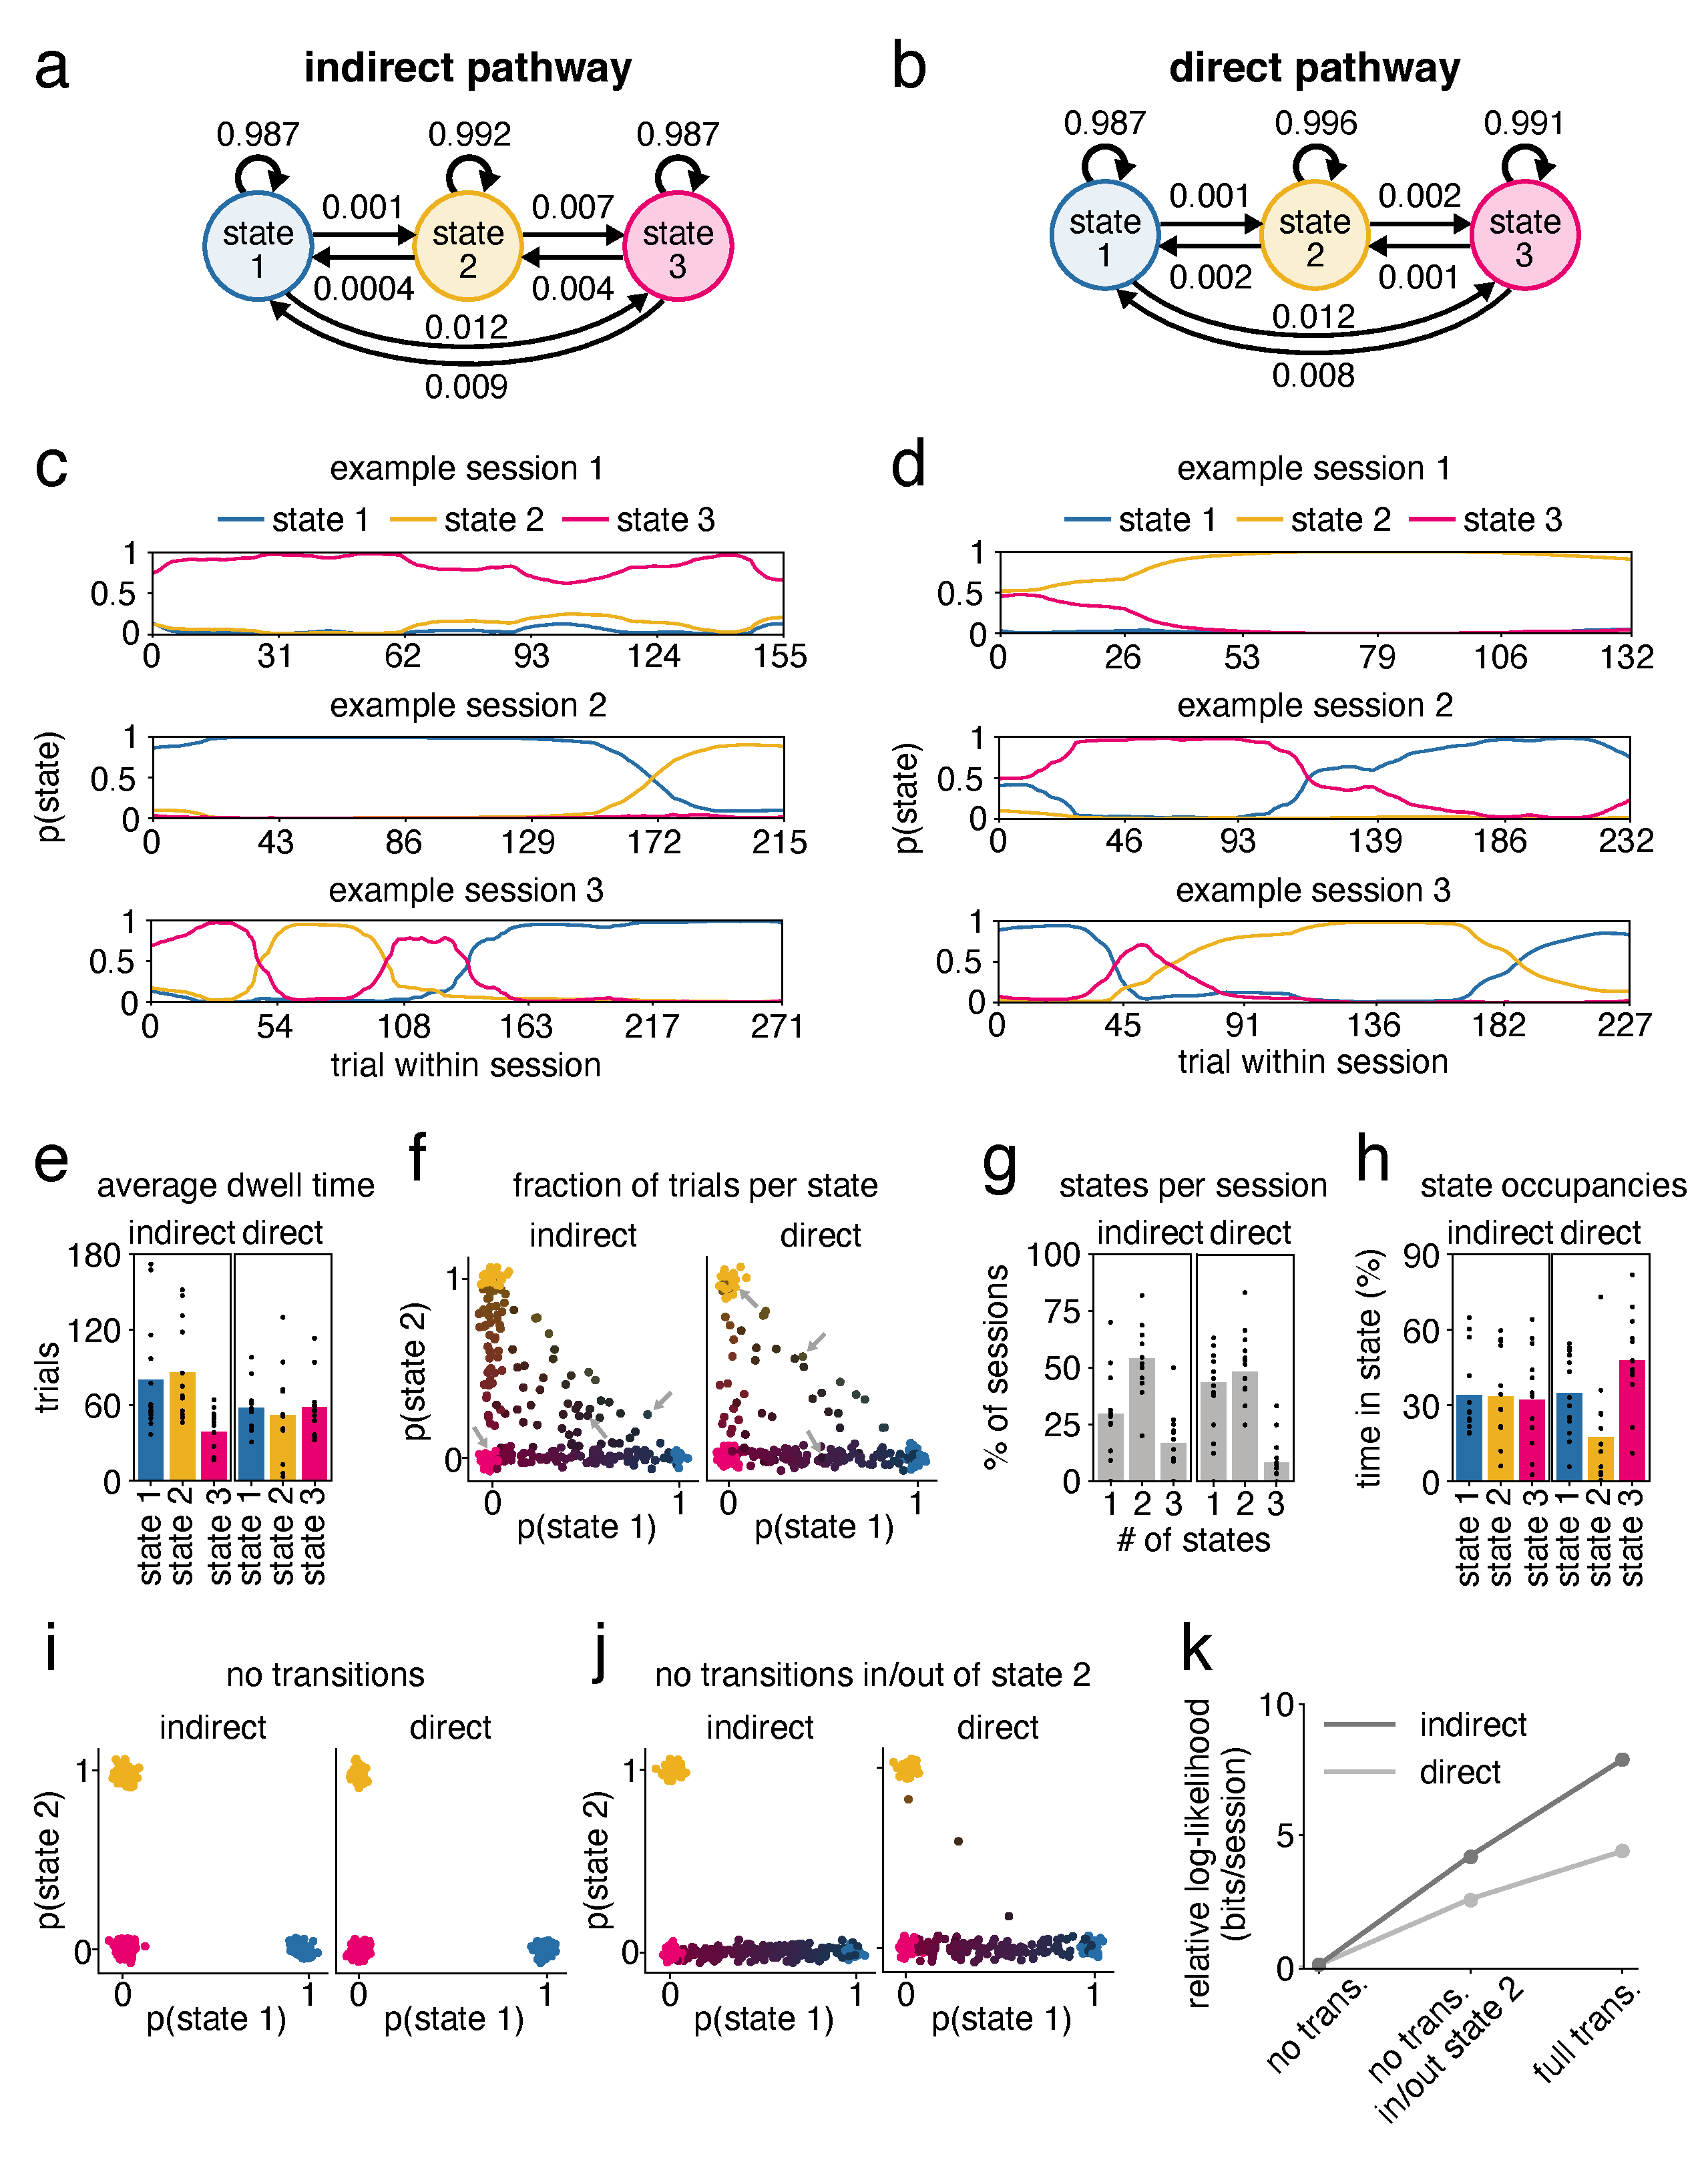
\includegraphics[width=0.90\linewidth]{ch2-glmhmm/glmhmm-figures/Fig7.pdf}
    \caption[Diversity across sessions in the timing and number of GLM–HMM state transitions]{\textbf{Diversity across sessions in the timing and number of GLM–HMM state transitions.} (a) Transition probabilities for the indirect pathway group. (b) Same as a but for the direct pathway group. (c) The posterior probability of being in each state for each trial for 3 example sessions from a mouse in the indirect pathway group. (d) Same as c but for two mice from the direct pathway group. (e) Dwell times showing the average consecutive number of trials that the mice spent in each state for mice with indirect (left; range 39-86 trials, average session length 202 trials) and direct (right; range 52-59 trials, average session length 185 trials) pathway}
    \label{fig:glmhmm:7}
  \end{center}
  \vspace{-1.5cm}
\end{figure}
\begin{figure}[t!]
  \contcaption{inhibition. Black dots show averages for individual mice (n=13 mice for both groups). (f). The fraction of trials that the mice spent in each state in each session. Each dot represents an individual session (n=271, indirect pathway; n=266, direct pathway). Color-coding reinforces the state composition of each session (e.g. blue indicates the mouse spent 100\% of the session in state 1). A small amount of Gaussian noise was added to the position of each dot for visualization purposes. Grey arrows identify the example sessions shown in c and d. (g) The fraction of sessions in which the mice entered one, two, or all three states. Gray bars denote the average fraction of sessions for all mice. Black dots show averages for individual mice (n=13 mice for both groups). (h) Time spent in each state represented as a percentage of total trials for mice inhibited in the indirect pathway (left) and direct pathway (right). Colored bars denote the average state occupancies across all mice. Black dots show averages for individual mice (n=13 mice both groups). (i) Same as f except state assignments were obtained from a model in which the transition probabilities were restricted to disallow transitions between states (i.e. all off-diagonal transition probabilities equal zero; see Methods). (j) Same as f except state assignments were obtained from a model in which transitions were disallowed between state 2 and the other states. (k) Comparison of the cross-validated log-likelihood of the data when fitting GLM-HMMs with the reduced models from i and j, relative to the log-likelihood of the full model, in bits per session. 
 }% Continued caption
\end{figure}

While individual sessions were heterogeneous in terms of their state occupancies, averaged across sessions, the posterior probability of being in each state tended to be stable across trials (Fig. \ref{fig:glmhmm:7}e and Extended Data Fig. \ref{fig:ap1:ext8}a,b). Model simulations recapitulated these state transition characteristics, including dwell times and state occupancies (Extended Data Fig. \ref{fig:ap1:ext9}), further indicating our model captures latent structure in our data.

One notable exception in the stability of posterior probabilities of each state across time was an increase in state 3 probability toward the end of a session (Extended Data Fig. \ref{fig:ap1:ext8}a), potentially reflecting a decrease in task engagement related to reward satiety. Consistent with a relationship to satiety, within-session transitions into state 3 were associated with higher amounts of previously accumulated reward and higher preceding rates of reward (Extended Data Fig. \ref{fig:ap1:ext8}c–f). In addition, while the posterior probability of each state showed minimal modulation surrounding a rewarded trial, the probability of state 3 was much more likely surrounding trials with excess travel (Extended Data Fig. \ref{fig:ap1:ext8}g–j), an indicator of non-goal-directed movement and task disengagement. Indeed, the probability of state 3 gradually increased and decreased approximately 25 trials before and following excess travel trials, consistent with the average dwell time for state 3 (Fig. \ref{fig:glmhmm:7}e).

Given the presence of sessions in which mice occupied a single state, we considered model variants that disallowed within-session state transitions. Our goal was to determine if these variant models could provide a better explanation of the data, or alternatively, if within-session state transitions are in fact an important structural feature for explaining the data. In one model variant, we disallowed transitions between states entirely (Fig. \ref{fig:glmhmm:7}k). In the other, we tested the possibility that state 2, which is unique in the strength of its laser weight, captured a session-specific feature of inhibition by disallowing transitions in and out of that state (Fig. \ref{fig:glmhmm:7}l). Using cross-validation, we found that neither alternative model explained the data as well as a model with unrestricted transitions (Fig. \ref{fig:glmhmm:7}m), indicating that within-session transitions between states was an important feature of the model.

